
%(BEGIN_QUESTION)
% Copyright 2012, Tony R. Kuphaldt, released under the Creative Commons Attribution License (v 1.0)
% This means you may do almost anything with this work of mine, so long as you give me proper credit

Write the equation describing the behavior of this pneumatic controller, assuming the PV and SP bellows are equal area (1.3 in$^{2}$), the output bellows has an area of 2.6 in$^{2}$, the fulcrum is precisely mid-point on the lever, and the supply pressure is 22 PSI:

$$\includegraphics[width=15.5cm]{i03756x01.eps}$$

Next, identify at least two different ways to {\it increase the gain} of this proportional-only pneumatic controller, if you could change any aspect of its construction:


\vskip 20pt \vbox{\hrule \hbox{\strut \vrule{} {\bf Suggestions for Socratic discussion} \vrule} \hrule}

\begin{itemize}
\item{} Explain why it is important to determine whether the mechanism is {\it force-balance} or {\it motion-balance} in your analysis.
\item{} Suppose someone suggested to you that the gain of this controller might be increased by enlarging the orifice.  Explain why this would have no effect on gain.
\item{} Suppose someone suggested to you that the gain of this controller might be increased by lengthening the lever (equally on both sides of the fulcrum) ``so that the baffle was more sensitive to motion.''  Explain why this would have no effect on gain.
\end{itemize}

\underbar{file i03756}
%(END_QUESTION)





%(BEGIN_ANSWER)

One way to increase gain is to move the fulcrum to the right (closer to the output bellows).

%(END_ANSWER)





%(BEGIN_NOTES)

$$m = 0.5 (\hbox{SP} - \hbox{PV}) + b$$

%INDEX% Control, proportional: pneumatic force-balance controller

%(END_NOTES)


